We implemented the model on a mesoscale mouse connectome,
which comprises of 213 fine areas,
grouped into 13 coarse areas,
along with measured connection strengths between the subcortices \cite{Oh2014}.
We used these coarse areas as the sets $C$ (\cref{eq:chimera,eq:metastability}) for chimera and metastability analyses.
We reduced the connection strengths to those with sufficient certainty ($p < 0.01$), and segmented as follows:
\begin{equation}
  \label{eq:mouse_segmentation}
  G_{j k}
  =
  \begin{cases}
    0 \text{ if } O_{j k} < 10^{-4}, \\
    1 \text{ if } 10^{-4} \leq O_{j k} < 10^{-2}, \\
    2 \text{ if } 10^{-2} \leq O_{j k} < 1, \\
    3 \text{ if } 1 \leq O_{j k},
  \end{cases}
\end{equation}
where $O_{j k}$ is the raw connection strength provided by \cite{Oh2014}.
We performed this simplification to match the analysis of Santos \etal more closely \cite{Santos2017}.

We show $G$ in \cref{fig:mouse_connectome}, and break it down into its inter- and intra-connections in \cref{fig:primes}.
This brain network is a small-world network \cite{Oh2014},
a graph topology which lends itself well to the development of chimera states, as it facilitates nonlocal coupling \cite{Hizanidis2016}.

\begin{figure*}[ht]
  \centering
  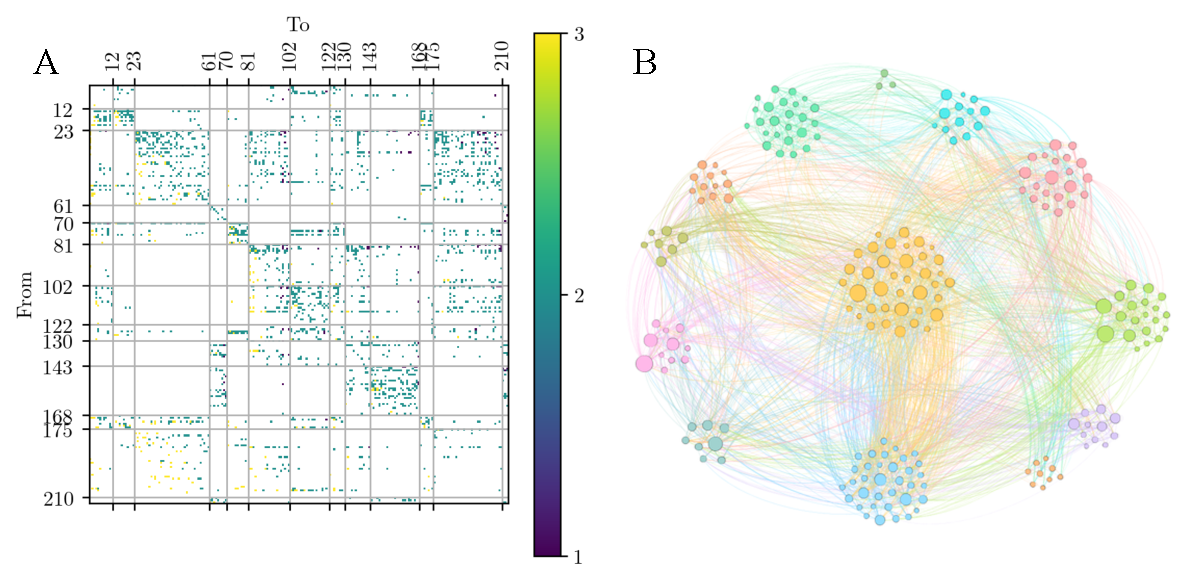
\includegraphics[width=\textwidth]{figure/network.pdf}
  \caption[Mouse connectome]{A. A matrix representation of the mouse connectome, with strengths as defined by \cref{eq:mouse_segmentation}.
    The cortices represented are, left to right (top to bottom),
    the striatum,
    the olfactory areas,
    the isocortex,
    the crebellar cortex,
    the hippocampal formation,
    the midbrain,
    the hypothalamus,
    the pallidum,
    the pons,
    the medulla,
    the cortical subplate,
    the thalamus,
    and the cerebellar nuclei.
    B. An embedding of the graph.
    Edge colors indicate the source location.
  }
  \label{fig:mouse_connectome}
\end{figure*}

Another benefit to this network is that it is comparatively accurate and complete.
Given the complexity of brains, creating an accurate structural or functional connectome is extremely difficult.
It has yet to be done to a large-scale extent in humans, and was only recently done in mice.
Moreover, as mice are common analogues for humans in laboratory settings, the mouse seemed a fitting ``guinea pig'' for the creation of chimera states.

\begin{figure}[ht]
  \centering
  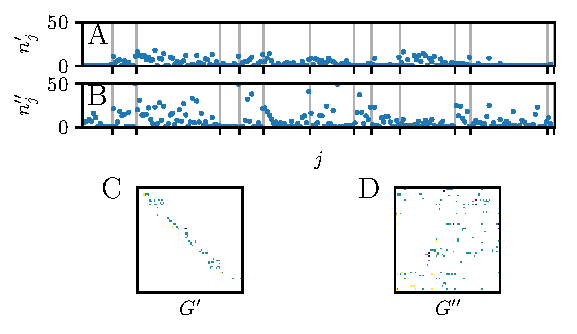
\includegraphics[width=0.5\textwidth]{figure/primes_100dpi.pdf}
  \caption[Network breakdown]{A breakdown of the network.
    A.\ \& B.\ show $n_{j}'$ and $n_{j}''$, effectively the number of nonzero elements in the $j$th row of $G'$ and $G''$, respectively.
    C.\ \& D.\ show $G'$ and $G''$, which are $G$ (\cref{fig:mouse_connectome} A) only within and between cortices, respectively.
  }
  \label{fig:primes}
\end{figure}

\begin{figure}[ht]
  \centering
  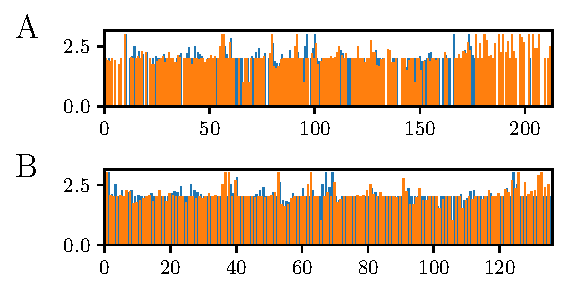
\includegraphics[width=0.5\textwidth]{figure/g_over_n_100dpi.pdf}
  \caption[Average strengths]{The average connection strengths for each neuron $j$, within cortices (blue) and between them (orange).
    A.\ All of the subcortices.
    B.\ All of the subcortices for which neither intra- nor inter-cortical average strength was 0.
  }
  \label{fig:average_strengths}
\end{figure}

%%% Local Variables:
%%% mode: latex
%%% TeX-master: "../../ms"
%%% End:
